\lab{Total Variation and Image Processing}{Total Variation and Image Processing}
\label{lab:tv_images}
\objective{Minimizing an energy functional is equivalent to solving the resulting Euler-Lagrange equations.  We introduce the method of steepest descent to solve these equations, and apply this technique to a denoising problem in image processing.}



\begin{enumerate}
\item Derive application-specific EL equations
\item Algorithm assumes smoothness.
Other theorems/algorithms have been developed using convex analysis, due to the recognition that the image might not be best represented by a smooth function $u:[0,1]\times [0,1] \to \mathbb{R}$. 
\item Code naive implementation using numpy
\item Analyze efficiency. 
Code with cython/numexpr?
\end{enumerate}

\section*{The Gradient Descent method}
Consider an energy functional $E[u]$, defined over a collection of admissible functions $u:\Omega \subset \mathbb{R}^n \to \mathbb{R}$. 
We suppose the energy functional $E$ has the form 
\[E[u] = \int_{\Omega} L(x,u,\nabla u) \, dx\]
where $L = L(x,y,w)$ is a function $\mathbb{R}^n \times \mathbb{R} \times \mathbb{R}^n \to \mathbb{R}$. 
A standard result from the calculus of variations states that a minimizing function $u^*$ satisfies the Euler-Lagrange equation
\begin{align}
L_y - {\rm div}\,(L_w) &= 0.	\label{EL:multivar_domain}
\end{align}

This equation is typically an elliptic PDE, possessing boundary conditions associated with  restrictions on the class of admissible functions $u$.
To more easily compute $\eqref{EL:multivar_domain}$, we may consider a related parabolic PDE:
\begin{align}
	\begin{split}
	&{ } u_t = -(L_y - {\rm div}\, L_w),\\
	&{ } u(x,t=0) = u_0(x).
	\end{split} \label{grad_desc_pde}
\end{align}
A steady state solution of \eqref{grad_desc_pde} does not depend on time, and thus is a solution of the Euler-Lagrange equation. 
In practice, it is often easier to evolve an initial guess $u_0$ using \eqref{grad_desc_pde}, stopping whenever its steady state is well-approximated, then to solve \eqref{EL:multivar_domain} directly. 

\begin{example}
Consider the energy functional 
\[ E[u] = \int_{\Omega} \|\nabla u\|^2 \, dx,\]
where the class of admissible functions $u$ satisfy appropriate Dirichlet conditions on $\partial \Omega$. 
The minimizing function $u^*$ satisfies the Euler-Lagrange equation
\[-{\rm div}\, \nabla u	= - \triangle u = 0.\]
The related PDE (called the gradient descent flow) is the well-known equation
\[u_t = \triangle u\]
describing heat flow.
\end{example}

The previous example brings to mind an interesting question: The Euler-Lagrange equation could equivalently be described as $\triangle u = 0$, leading to the PDE $u_t = -\triangle u$. 
Since this (backward) heat equation is ill-posed, it will not be helpful in our search for a steady-state. 

Let us take the time to put \eqref{grad_desc_pde} on a more rigorous footing. 
Recalling the derivation of the Euler-Lagrange equation, we note that 
\begin{align*}
		\delta E(u;v) &= \left.\frac{d}{dt}E(u + tv)\right|_{t=0},\\
		&= \int_{\Omega} (L_y(u) - {\rm div}\, L_w(u)) v\, dx
\end{align*}
for each $u$ and each admissible perturbation $v$.
We can now employ the Cauchy-Schwarz inequality: 
\begin{align*}
	|\delta E(u;v)| &= | \langle L_y(u) - {\rm div}\, L_w(u), v \rangle_{L^2(\Omega)} |,\\
	&\leq \|L_y(u) - {\rm div}\, L_w(u)\| \cdot \| v \|,
\end{align*}
with equality iff $v =\alpha u$ for some $\alpha \in \mathbb{R}$. 
This implies that the ``direction" 
$v = L_y(u) - {\rm div}\, L_w(u)$
maximizes $\delta E(u)$. 
Similarly,
\[v = -(L_y(u) - {\rm div}\, L_w(u))\]
 points in the direction of steepest descent, and the flow described by \eqref{grad_desc_pde} tends to move toward a state of lesser energy. 


\subsection*{Example: Finding the curve that surface of revolution minimizes surface area}
Consider the collection of smooth curves defined on $[a,b]$, with fixed end points $y(a) = y_a$, $y(b) = y_b$. The surface obtained by revolving a curve $y(x)$ about the $x$-axis has area given by the functional 
\[A[y] = \int_a^b y 2 \pi \sqrt{1 + (y')^2} \, dx.
\]
The Euler-Lagrange equation is 
\begin{align}
	\begin{split}
	0 &= 1 - y \frac{y''}{1 + (y')^2} , \\
	&= 1 + (y')^2 - y y'',
	\end{split}\label{tv_images:SA_EL_equation}
\end{align}
and the resulting gradient descent flow is given by
\begin{align}
	\begin{split}
	&{ } u_t = -1 - (y')^2 + y y'', \\
	&{ } u(a,t) = y_a, \quad u(b,t) = y_b,\\
	&{ } u(x,0) = g(x),
	\end{split}\label{tv_images:SA_flow}
\end{align}
where $g(x)$ is an appropriate initial guess.

Consider a second-order order discretization in space, with a simple forward Euler step in time. Let us impose the conditions $y(-1) = 1$, $y(1) = 7$. We begin by creating a grid to approximate the solution on: 
\begin{lstlisting}
import numpy as np

a, b = -1, 1.
alpha, beta = 1., 7.
####  Define variables x_steps, final_T, time_steps  ####
delta_t, delta_x = final_T/time_steps, (b-a)/x_steps
x0 = np.linspace(a,b,x_steps+1)
\end{lstlisting}

Often there is a stability condition required for a numerical scheme. 
One that is common for this discretization is that $\frac{\triangle t}{(\triangle x)^2} \leq \frac{1}{2}$.  
We continue by checking that this condition is satisfied, and setting our initial guess to be the straight line connecting the end points. 

\begin{lstlisting}
# Check a stability condition for this numerical method
if delta_t/delta_x**2. > .5:
	print "stability condition fails"
	
u = np.empty((2,x_steps+1))
u[0]  = (beta - alpha)/(b-a)*(x0-a)  + alpha
u[1] = (beta - alpha)/(b-a)*(x0-a)  + alpha
\end{lstlisting}

Finally, we define the right hand side of our difference scheme, and time step until we 
achieve a desired accuracy. 
\begin{lstlisting}
def rhs(y):
	# Approximate first and second derivatives to second order accuracy.
	yp = (np.roll(y,-1) - np.roll(y,1))/(2.*delta_x)
	ypp = (np.roll(y,-1) - 2.*y + np.roll(y,1))/delta_x**2.
	# Find approximation for the next time step, using a first order Euler step
	y[1:-1] -= delta_t*(1. + yp[1:-1]**2. - 1.*y[1:-1]*ypp[1:-1])


# Time step until successive iterations are close
iteration = 0
while iteration < time_steps:
	rhs(u[1])
	if norm(np.abs((u[0] - u[1]))) < 1e-5: break
	u[0] = u[1]
	iteration+=1

print "Difference in iterations is ", norm(np.abs((u[0] - u[1])))
print "Final time = ", iteration*delta_t
\end{lstlisting}

\begin{figure}
\centering
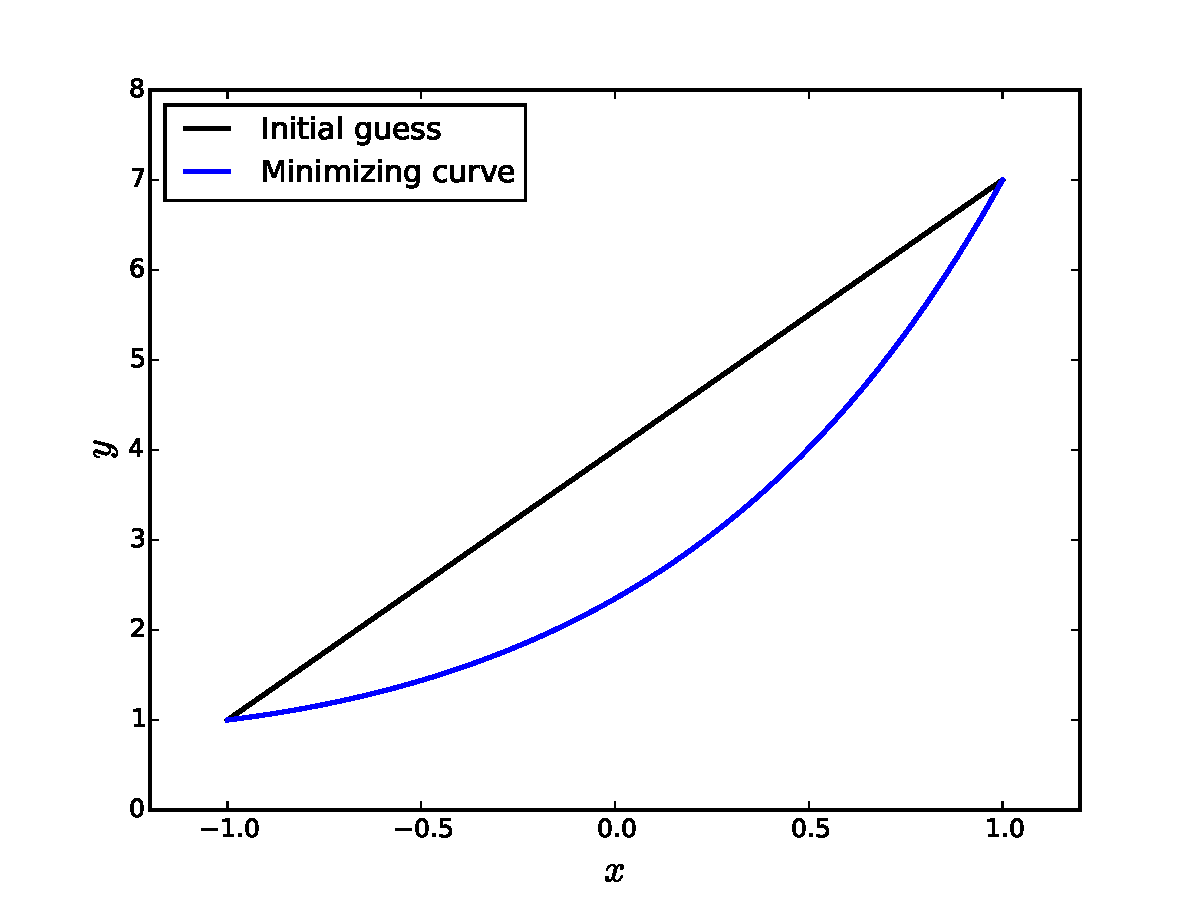
\includegraphics[width=\textwidth]{min_surface_area.pdf}
\caption{The solution of \eqref{tv_images:SA_EL_equation}, found using the gradient descent flow \eqref{tv_images:SA_flow}.}
\label{fig:tv_images:SA_image}
\end{figure}


\section*{Image Processing}
\[
\frac{\lambda}{2} \int_{\Omega} | \nabla u |^2 + \frac{1}{2} \int_{\Omega}(u - f)^2
\]
\begin{align*}
L = L(x,\nabla u, u) &= \frac{1}{2}(u-f)^2 + \frac{\lambda}{2} | \nabla u|^2,\\
&= \frac{1}{2}(u-f)^2 + \frac{\lambda}{2} (u_x^2 + u_y^2)^2.
\end{align*}







\section*{Total Variation Method}
We represent an image by a function $u:[0,1]\times[0,1] \to \mathbb{R}$. 
A $C^1$ function $u:\Omega \to \mathbb{R}$ has bounded total variation on $\Omega$ ($BV(\Omega)$) if $\int_{\Omega} u < \infty$; $u$ is said to have total variation $\int_{\Omega} u$.  Intuitively, the total variation of an image $u$ increases when noise is added. 

The total variation approach was originally introduced by Ruding, Osher, and Fatemi\footnote{L. Rudin, S. Osher, and E. Fatemi, ``Nonlinear total variation based noise removal algorithms'', \emph{Physica D.}, 1992.}. It was formulated as follows: given a noisy image $f$, we look to find a denoised image $u$ minimizing 
\begin{align}
\int_{\Omega} |\nabla u(x)|\, dx \label{tv_images:tv}
\end{align}
subject to the constraints 
\begin{align}
	&{ } \int_{\Omega} u(x) \, dx = \int_{\Omega} f(x)\, dx, \label{tv_images:same_mean}\\
	&{ } \int_{\Omega} |u(x) - f(x)|^2\, dx = \sigma |\Omega|.\label{tv_images:aprior_variance}
\end{align}
Intuitively, \eqref{tv_images:tv} penalizes fast variations in $f$ - this functional together with the constraint \eqref{tv_images:same_mean} has a constant minimum of $u = \frac{1}{|\Omega|}\int_{\Omega} u(x) \, dx$. This is obviously not what we want, so we add a constraint \eqref{tv_images:aprior_variance} specifying how far $u(x)$ is required to differ from the noisy image $f$.  More precisely, \eqref{tv_images:same_mean} specifies that the noise in the image has zero mean, and \eqref{tv_images:aprior_variance} requires that a variable $\sigma$ be chosen a priori to represent the standard deviation of the noise. 

Solving for the original denoised image $u$ is a difficult inverse problem; some information about the image is irretrievably lost when the noise is introduced. A priori information can however be used to guess at the structure of the original image.  For example, in this problem $\sigma$ represents our best guess on how much noise was added to the image. $\sigma$ is known as a regularization parameter in inverse problem theory. 

Chambolle and Lions proved that the model introduced by Rudin, Osher, and Fatemi can be formulated equivalently as 
\begin{align}
\min_{u \in BV(\Omega)} \int_{\Omega} | \nabla u(x)|\, dx +\frac{\lambda}{2}\|u-f\|_{L^2(\Omega)}^2,	
\end{align}
where $\lambda >0$ is a fixed regularization parameter\footnote{A. Chambelle and P.-L. Lions, ``Image recovery via total variation minimization and related problems", \emph{Numer. Math.}, 1997.}.













